\documentclass[a4paper, 11pt]{article}
\usepackage[utf8]{inputenc}
\usepackage{graphicx,wrapfig,subfigure,amsmath,amssymb,epsfig,bm}
\usepackage{listings,textcomp,color,geometry}
\geometry{hmargin=2cm, vmargin=2cm}

\def\Box{\mathord{\dalemb{7.9}{8}\hbox{\hskip1pt}}}
\def\dalemb#1#2{{\vbox{\hrule height.#2pt
        \hbox{\vrule width.#2pt height#1pt \kern#1pt \vrule width.#2pt}
        \hrule height.#2pt}}}

\def\eop{\mathcal{E}}
\def\bop{\mathcal{B}}
\def\ba{\begin{eqnarray}}
\def\ea{\end{eqnarray}}
\def\be{\begin{equation}}
\def\ee{\end{equation}}
\def\tr{{\rm tr}}
\def\Var{{\rm Var}}
\def\gtorder{\mathrel{\raise.3ex\hbox{$>$}\mkern-14mu
             \lower0.6ex\hbox{$\sim$}}}
\def\ltorder{\mathrel{\raise.3ex\hbox{$<$}\mkern-14mu
             \lower0.6ex\hbox{$\sim$}}}

\def\bb{{\mathfrak b}}
\newcommand{\ellb }{\boldsymbol{\ell }}

% Personal colors defined here
\newcommand{\skn}[1]{{\color{red}#1}}
\newcommand{\TIB}[1]{{\color{blue}#1}}

\begin{document}

\title{\textbf{ACTPol Cookbook}}
\author{The ACTPol collaboration}
\maketitle

The goal of this document is not to be exhaustive, not to be complete, not
to be free of typos, not to be circulated outside the AdvACT collaboration.
It is supposed to be a living document.  Choose your color for
editing/asking clarification in other people sections: \skn{Sigurd}, \TIB{Thibaut}.

\section{TOD cut and calibration}

\section{Beams, pointing model, time constant}

\section{Point sources, mask and cluster studies}


\section{Map making (Sigurd and Simone)}

\section{Power spectra (Thibaut and Steve)}

We both use the MASTER algorithm for Power Spectrum estimation. We compute pseudo-power spectrum and then correct for the effect of the window function, beam and filter applied to the data. Other methods exist for power spectrum estimation. Because they contain $10^{7}-10^{8}$ pixels, optimal methods are hard to implement for the ACTPol maps.

\subsection{Basic principles}\label{subsec:PSbasis}

The output of the map making pipeline is a set of maps in CAR pixellization: $T(\bm{x}), Q(\bm{x}), U(\bm{x})$, a set of hit count maps and an estimation of the covariance (T,Q,U) of the noise. The power spectrum pipeline uses the hit count map for weighting the data, but  does not yet use this covariance.
Enki provides (T,Q,U) as an individual fit file, while Ninkasi output the maps separately, tools exist in Enlib to convert from one format to the other. 

The maps consist of four splits for s13, s14, s15 and two splits for s16. This format has been chosen to ensure  approximate even coverage for each of the splits. 

The main output of the power spectrum pipeline is  the TT, TE, TB, EE, EB, BB cross spectra. They are average of the $N_{s}(N_{s}+1)/2$ individual cross spectra obtained by cross correlating different splits  ($N_{s}$ is the number of splits). The $N_{s}$ auto spectra are  used to estimate the noise properties of the data. 

Let us start this with a simple data model for temperature anisotropies, we will use the flat sky approximation

\ba
\tilde{T}_{i}(\bm{x}) &=& \int d\bm{x'} b( \bm{x}-\bm{x'}) W(\bm{x'}) T(\bm{x'})+W( \bm{x}) n_{i} (\bm{x})  \\
\ea
Here $b( \bm{x})$ represent the effect of the beam and $W( \bm{x})$ is the window function applied to the data. The window function is given by the product of a point source mask, the hit count map and an apodization function. The Fourier transform of this map is given by
\ba
\tilde{T}_{i}(\bm{\ell}) &=& \int d\bm{\ell'} W (\bm{\ell}-\bm{\ell'}) \left[ b(\bm{\ell'}) T(\bm{\ell'}) + n_{i}(\bm{\ell'})\right] \label{eq:Tfourier}
\ea
An estimator for the two dimensional cross power spectrum $C(\bm{\ell})=\langle T(\bm{\ell}) T^{*}(\bm{\ell}) \rangle $ can be simply written  
\ba
\tilde{C}(\bm{\ell})= \tilde{T}_{i}(\bm{\ell}) \tilde{T}^{*}_{j}(\bm{\ell})
\ea
However this estimator is biased $\langle \tilde{C}(\bm{\ell}) \rangle \neq C(\bm{\ell})$, indeed
\ba
\langle \tilde{C}(\bm{\ell}) \rangle &=& \langle  \tilde{T}_{i}(\bm{\ell}) \tilde{T}^{*}_{j}(\bm{\ell}) \rangle \\
&=& \int d\bm{\ell'} | W (\bm{\ell}-\bm{\ell'})|^{2}b^{2}(\bm{\ell'})  C(\bm{\ell'})
\ea
where we used the fact that the noise on different splits is uncorrelated $ \langle n_{i}(\bm{\ell}) n_{j}(\bm{\ell}) \rangle=0$. When we display two dimensional power spectra, we are looking at this quantity. In order to get an unbiased estimator, we need to invert this equation. So far, I used the continuous limit to write down the equation system. In reality the number of modes is finite and this equation can be rewritten as a matrix equation
\ba
\langle \tilde{C}_{\bm{\ell}} \rangle= \sum_{\bm{\ell}'} M_{\bm{\ell}, \bm{\ell'}}  C_{\bm{\ell'}}
\ea 
Inverting this equation is then equivalent to finding the inverse of the matrix $ M_{\bm{\ell}, \bm{\ell'}} $. In practice however, the matrix is not well conditionned, and its inverse does not exist. The physical reason for which this matrix can not be inverted is quiet clear. If you observe only a fraction of the sky, you can not distinguish between close-by Fourier modes, this is equivalent to say that you have limited resolution in harmonic space. In practice, what we do is to bin the matrix and the power spectrum, and turn the equation system into
\ba
\langle \tilde{C}_{b} \rangle= \sum_{b'} M_{b, b'}  C_{b'}
\ea 
Our final estimate for the power spectrum is then
\ba
\hat{C}_{b}= (M_{b, b'})^{-1} \tilde{C}_{b'} 
\ea
This estimator is unbiased. Computing and inverting $M_{b, b'}$ is really the name of the game of power spectrum estimation. It is by far the most expensive step in the power spectrum pipeline.

\subsection{Polarization data in the Flat-Sky approximation}

The polarization field can be written as  a $2\times2$ symmetric, trace free, tensor 
\ba
P_{ab}(\bm{x})= \frac{1}{2}
\begin{pmatrix} 
Q(\bm{x}) & 
U(\bm{x}) \cr
U(\bm{x}) & 
-Q(\bm{x}) \cr
\end{pmatrix} 
\ea
This form ensures that Q and U transform as expected under a coordinate transformation (imagine for example a rotation of your detectors' array).
Any $2\times2$ symmetric, trace free, tensor can be uniquely decomposed in two parts
\ba 
\eop_{ab} A=(-\partial_{a}\partial_{b}+ \frac{1}{2}\delta_{ab} \nabla^{2})A \ ; \ \bop_{ab}B=\frac{1}{2} (\epsilon_{ac}\partial^{c}\partial_{b} + \epsilon_{bc}\partial^{c}\partial_{a})B
\ea
where A and B are scalar functions. Since the $e^{i\bm{\ell} \bm{x}}$ provide a basis for a scalar function in the plane, we define
\ba
(^{E}e^{i\bm{\ell}\bm{x}})_{ab} &=& N_{\bm{\ell}} \eop_{ab} (e^{i\bm{\ell}\bm{x}})= N_{\bm{\ell}} ( \ell_{a}\ell_{b}- \frac{\bm{\ell}^{2}}{2}\delta_{ab})e^{i\bm{\ell}\bm{x}} \\
(^{B}e^{i\bm{\ell}\bm{x}})_{ab} &=& M_{\bm{\ell}}\bop_{ab} (e^{i\bm{\ell}\bm{x}})=- \frac{M_{\bm{\ell}}}{2} (\epsilon_{ac}\ell^{c}\ell_{b} + \epsilon_{bc}\ell^{c}\ell_{a}) e^{i\bm{\ell}\bm{x}}
\ea
The normalization coefficient $N_{\bm{\ell}}$ is chosen in order to ensure the orthogonality relation.
\ba
\int d^{2}x (^{E}e^{i\bm{\ell}\bm{x}})^{*}_{ab} (^{E}e^{i\bm{\ell}'\bm{x}})^ {ab} = \delta( \bm{\ell}-\bm{\ell}')
\ea
we can expand the polarization field on this basis
\ba
P_{ab}(\bm{x}) &=& \frac{1}{\sqrt{2}} \int d\bm{\ell} E(\bm{\ell}) (^{E}e^{i\bm{\ell}\bm{x}})_{ab} +B({\bm{\ell}}) (^{B}e^{i\bm{\ell}\bm{x}})_{ab} \\
 E({\bm{\ell}}) &=& \frac{2}{\ell^{2}} \int d^{2}x   P_{ab}(\bm{x})   \eop^{ab}(e^{-i\bm{\ell}\bm{x}}) \\
 B({\bm{\ell}}) &=& \frac{2}{\ell^{2}} \int d^{2}x   P_{ab}(\bm{x})  \bop^{ab}(e^{-i\bm{\ell}\bm{x}}) 
\ea
this is equivalent to the spin formalism for polarization data
\ba
E({\bm{\ell}}) &=& Q(\bm{\ell}) \cos 2\phi_{\bm{\ell}}+U(\bm{\ell})\sin 2\phi_{\bm{\ell}}   \\
B({\bm{\ell}}) &=& -Q(\bm{\ell})\sin 2\phi_{\bm{\ell}} +U(\bm{\ell}) \cos 2\phi_{\bm{\ell}}  \\
E({\bm{\ell}}) \pm i B({\bm{\ell}})&=& e^{\mp 2i\phi_{\bm{\ell}}}(Q(\bm{\ell}) \pm i U(\bm{\ell}))
\ea
The Q and U maps geometry can also be read trivially from this set of equation, using a polarisation convention compatible with the output of the map maker, we have

\newcommand{\costwo}{\ensuremath{%
  \mathchoice{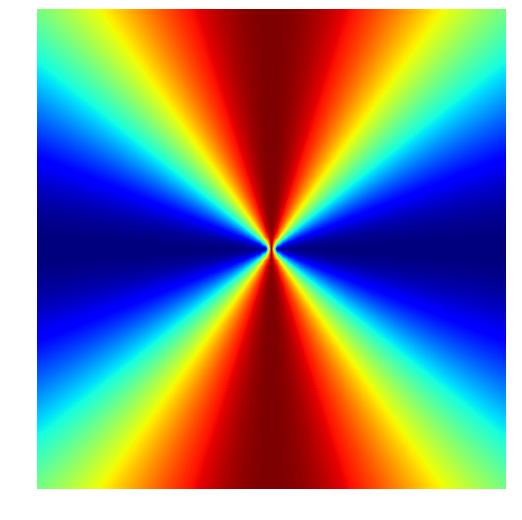
\includegraphics[height=4ex]{cos2.png}}
    {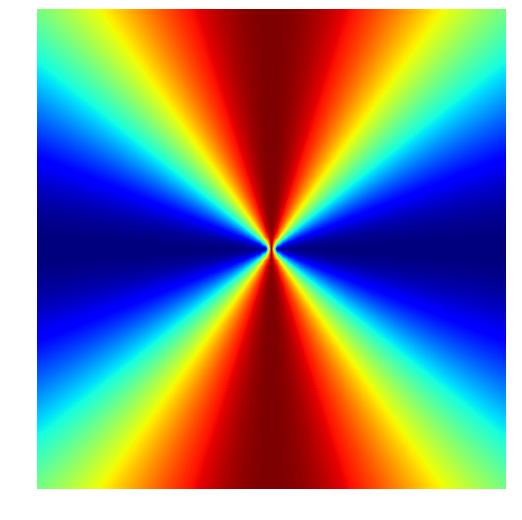
\includegraphics[height=2ex]{cos2.png}}
    {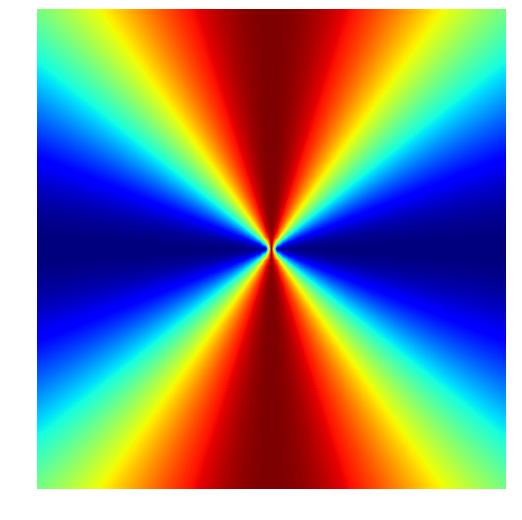
\includegraphics[height=1.5ex]{cos2.png}}
    {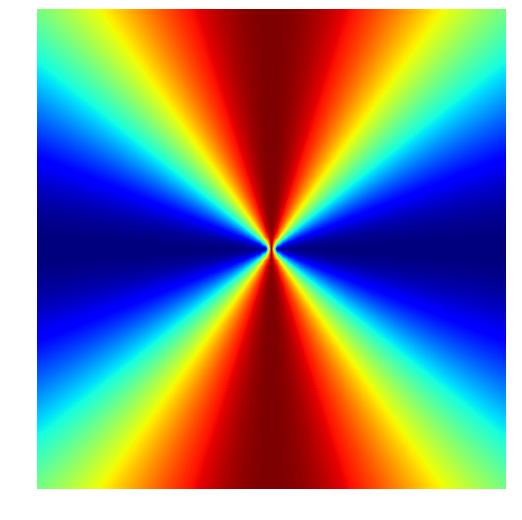
\includegraphics[height=1ex]{cos2.png}}
}}

\newcommand{\sintwo}{\ensuremath{%
  \mathchoice{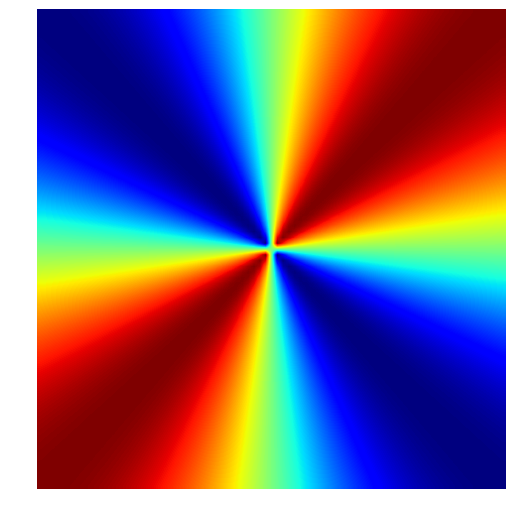
\includegraphics[height=4ex]{sin2.png}}
    {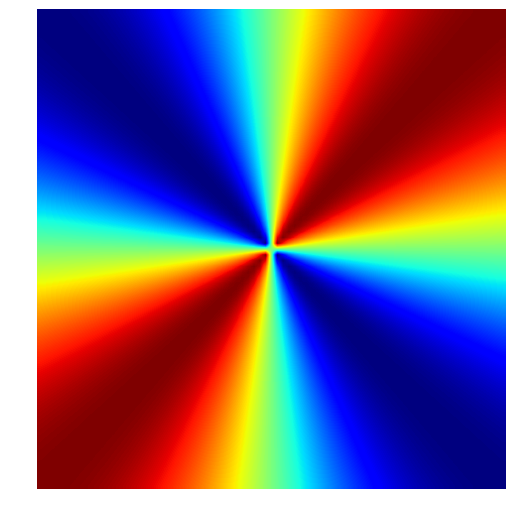
\includegraphics[height=2ex]{sin2.png}}
    {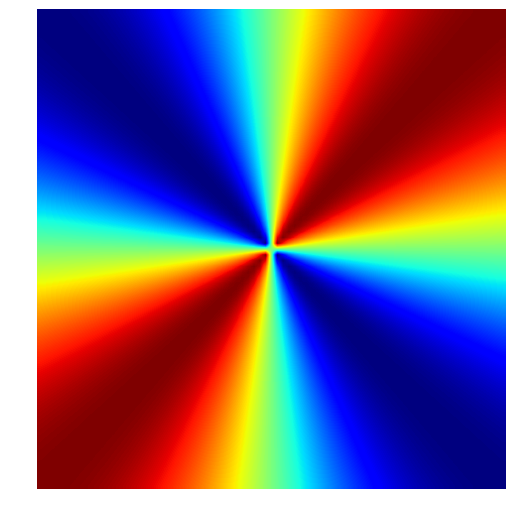
\includegraphics[height=1.5ex]{sin2.png}}
    {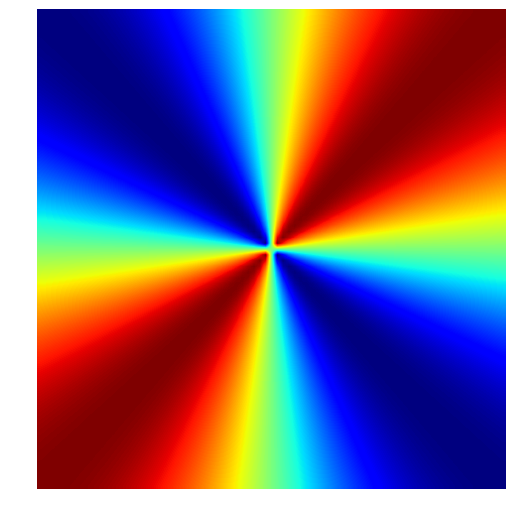
\includegraphics[height=1ex]{sin2.png}}
}}
\ba
Q(\bm{\ell}) &=& E(\bm{\ell}) \costwo - B(\bm{\ell}) \sintwo \\
U(\bm{\ell}) &=& E(\bm{\ell}) \sintwo + B(\bm{\ell}) \costwo
\ea
where we replace the cos and sin by a graphical representation. We can see that if the map is dominated by E modes  Q will have a '+' geometry and U will have a '$\times$' geometry.

\subsubsection{Mode coupling calculation }
We need to extend the mode coupling calculation presented in  \ref{subsec:PSbasis}, to polarization data.  We start by computing the Fourier transform of the Stokes component
\ba
\tilde{Q}_{i}(\bm{\ell}) &=& \int d\bm{\ell'} W (\bm{\ell}-\bm{\ell'}) \left[ b(\bm{\ell'}) Q(\bm{\ell'}) + n^{Q}_{i}(\bm{\ell'})\right]  \\
\tilde{U}_{i}(\bm{\ell}) &=& \int d\bm{\ell'} W (\bm{\ell}-\bm{\ell'}) \left[ b(\bm{\ell'}) U(\bm{\ell'}) + n^{U}_{i}(\bm{\ell'})\right] 
\ea
to simplify the equations and with no loss of generality we will ignore the noise term in the derivation. The observed E and B modes can be written
\ba
\tilde{E}({\bm{\ell}}) \pm i \tilde{B}({\bm{\ell}})&=& e^{\mp 2i\phi_{\bm{\ell}}}(\tilde{Q}(\bm{\ell}) \pm i \tilde{U}(\bm{\ell})) \\
&=& \int d\bm{\ell'} b(\bm{\ell'}) W(\bm{\ell}-\bm{\ell'})  [E({\bm{\ell}'}) \pm i B({\bm{\ell}'})]  e^{  \pm 2i (\phi_{\bm{\ell'}} - \phi_{\bm{\ell}})  }  
\ea
The estimated E (B) modes are then given by a mixture of E and B modes
\ba
\tilde{E}({\bm{\ell}})&=&  \int d\bm{\ell'} b(\bm{\ell'}) W(\bm{\ell}-\bm{\ell'})  [  E({\bm{\ell}'}) \cos  2(\phi_{\bm{\ell'}} - \phi_{\bm{\ell}})  - B({\bm{\ell}'}) \sin  2(\phi_{\bm{\ell'}} - \phi_{\bm{\ell}})  ]   \nonumber \\
\tilde{B}({\bm{\ell}}) &=&  \int d\bm{\ell'} b(\bm{\ell'}) W(\bm{\ell}-\bm{\ell'})  [  E({\bm{\ell}'}) \sin  2(\phi_{\bm{\ell'}} - \phi_{\bm{\ell}})  + B({\bm{\ell}'}) \cos  2(\phi_{\bm{\ell'}} - \phi_{\bm{\ell}})  ]   \nonumber \\
\ea
This is important. The amount of B modes in the map is much smaller than the amount of E modes. The observed B modes map will therefore be dominated by the leakage of E modes due to the window function (the partial sky coverage).
Following what we have done in \ref{subsec:PSbasis}, we can relate the estimated power spectrum to the unbiased power spectrum using a mode coupling matrix
\ba
 \begin{pmatrix}  \tilde{C}_{TE}({\bm{\ell}})\cr \tilde{C}_{TB}({\bm{\ell}})\cr \tilde{C}_{EE} ({\bm{\ell}})  \cr \tilde{C}_{EB} ({\bm{\ell}})  \cr \tilde{C}_{BB} ({\bm{\ell}}) \end{pmatrix} = \sum_{\bm{\ell'} }M_{\bm{\ell}, \bm{\ell'}}\begin{pmatrix}  C_{TE}({\bm{\ell}'})\cr C_{TB}({\bm{\ell}'})\cr C_{EE}({\bm{\ell}'})\cr C_{EB}({\bm{\ell}'})\cr C_{BB}({\bm{\ell}'})\cr  \end{pmatrix} 
\ea
\ba
M_{\bm{\ell}, \bm{\ell'}}= b^{2}(\bm{\ell'})  | W(\bm{\ell}-\bm{\ell'})|^{2} 
\begin{pmatrix} 
\cos \Delta_{\bm{\ell},\bm{\ell'}}  & 
-\sin \Delta_{\bm{\ell},\bm{\ell'}} &
0 & 
0 & 
0 & 
\cr
\sin \Delta_{\bm{\ell},\bm{\ell'}}  & 
\cos \Delta_{\bm{\ell},\bm{\ell'}}  &
0 & 
0 & 
0 & 
  \cr
0 & 
0 &
\cos^{2} \Delta_{\bm{\ell},\bm{\ell'}} & 
-2 \cos \Delta_{\bm{\ell},\bm{\ell'}}  \sin \Delta_{\bm{\ell},\bm{\ell'}} &
\sin^{2} \Delta_{\bm{\ell},\bm{\ell'}}  &  
 \cr
0 & 
0 &
\cos \Delta_{\bm{\ell},\bm{\ell'}}  \sin \Delta_{\bm{\ell},\bm{\ell'}} & 
\cos^{2} \Delta_{\bm{\ell},\bm{\ell'}}-\sin^{2} \Delta_{\bm{\ell},\bm{\ell'}} & 
-\cos \Delta_{\bm{\ell},\bm{\ell'}}  \sin \Delta_{\bm{\ell},\bm{\ell'}} & 
\cr
0 & 
0 &
\sin^{2} \Delta_{\bm{\ell},\bm{\ell'}}  & 
2 \cos \Delta_{\bm{\ell},\bm{\ell'}}  \sin \Delta_{\bm{\ell},\bm{\ell'}} & 
\cos^{2} \Delta_{\bm{\ell},\bm{\ell'}}  & 
\cr
\end{pmatrix}
\ea
With  $\Delta_{\bm{\ell},\bm{\ell'}}= 2(\phi_{\bm{\ell'}} - \phi_{\bm{\ell}})$. Again this matrix can not be inverted. Both the mode coupling matrix and the spectra need to be binned first.

\subsection{Flat sky vs Full sky}



\subsection{Azimuthal weighting}

\subsection{Prewithening}

\subsection{Cross frequencies and Cross seasons  power spectra}

\subsection{Planck calibration}

\subsection{Covariance matrix}


%An estimator of the two dimensional cross power spectrum is obtained by taking the average of each cross spectrum
%\ba
%\tilde{C}(\bm{\ell}) &=& \frac{1}{N_c}\sum_{i,k>i} \tilde{T}_{i}(\bm{\ell}) \tilde{T}_{k}(\bm{\ell}) \\
%N_c &=& \sum_{i,k>i} 1=  N_{s}(N_{s}+1)/2
%\ea
%Let us focus on a given pair of split 
 
\section{Lensing}

\subsection{Data prep}
\subsection{Sims}
\subsection{Kappa maps}
\subsection{Biases and Power spectra}
\subsection{Delensing}
\subsection{Likelihood}

For any T, E, B pair that we denote as $x$, the quadratic estimator starts off being wrong by some cosmology-dependent normalization (all $LM$ indices are suppressed),

$$
\langle \hat{x} \rangle = R_{x} \kappa_x 
$$

We correct by some fiducial cosmology letting the estimator be $\hat{\kappa}_x = \hat{x} / R^0_x$. This means the expected value is now,

$$
\langle\hat\kappa\rangle = \frac{R_x}{R^0_x}\kappa 
$$

Next, we calculate the power spectrum, but correct for the anticipated $N_1$ bias,

$$
\hat{C}_{xy}=\frac{1}{R^0_xR^0_y}\hat{x}\hat{y} - N_{1,xy}^0
$$

which leads to an expected theory power spectrum of,

$$
C_{xy}^{\mathrm{th}}=\frac{R_xR_y}{R^0_xR^0_y}C_{xy} + N_{1,xy} - N_{1,xy}^0
$$

Expanding the $R$'s and $N$'s about the fiducial by some parametrization $\boldsymbol{\theta}$,

\newcommand{\bth}{\boldsymbol{\theta}}
\newcommand{\bna}{\boldsymbol{\nabla}}

\begin{align*}
C_{xy}^{\mathrm{th}}&\approx\frac{R^0_xR^0_y+\bna^0_{\bth} (R_xR_y)\cdot (\bth-\bth_0)}{R^0_xR^0_y}C_{xy} + \bna^0_{\bth} N_{1,xy}\cdot (\bth-\bth_0) \\
&\approx C_{xy}+\bna^0_{\bth} \mathrm{ln}(R_xR_y)\cdot (\bth-\bth_0)C_{xy} + \bna^0_{\bth} N_{1,xy}\cdot (\bth-\bth_0)
\end{align*}

The Planck parametrization is $\bth=\{C_x, C_{xy}\}$ (the CMB and convergence spectra, respectively).

\subsubsection{Corrections}

\newcommand{\bell}{\boldsymbol{\ell}}
\newcommand{\bL}{\boldsymbol{L}}

For each polcomb in $\alpha=\{\mathrm{TT,TE,EE,EB}\}$, we calculate the normalization

$$
L^2A_{\alpha}^{-1}(\bL) = \int \frac{d^2\bell_1}{(2\pi)^2} f_{\alpha}(\bell_1,\bell_2)F_{\alpha}^0(\bell_1,\bell_2)
$$

Here, $F_{\alpha}^0(\bell_1,\bell_2)$ and $f_{\alpha}(\bell_1,\bell_2)$ are functions of the CMB power spectra. The former is always evaluated at the fiducial cosmology assumed in the main analysis. We calculate derivatives of the normalization with respect to CMB power spectra by shifting the amplitude in annuli of width $\Delta \ell$ of the respective 2D CMB power spectra that are used in $f_{\alpha}(\bell_1,\bell_2)$. For the TT case,

$$
R(\bL) \equiv L^2A_{TT}^{-1}(\bL) = \int \frac{d^2\bell_1}{(2\pi)^2} (C_{\ell_1}(\bL.\bell_1)+C_{\ell_2}(\bL.\bell_2))F_{TT}^0(\bell_1,\bell_2)
$$

$$
\frac{\partial R(\bL)}{\partial C_{\ell}} = \int \frac{d^2\bell_1}{(2\pi)^2} (\delta(\ell_1-\ell)(\bL.\bell_1)+(\delta(\ell_2-\ell)(\bL.\bell_2))F_{TT}^0(\bell_1,\bell_2)
$$

$$
\frac{\partial^2 R(\bL)}{\partial C^2_{\ell}} = 0
$$

Ignoring the N1 correction for now, we expand up to all orders in the product of $R$s, which only gives one additional term.

\begin{align*}
C_{xy}^{\mathrm{th}}&\approx\frac{R^0_xR^0_y+\bna_{\bth} (R_xR_y)\cdot (\bth-\bth_0)+\bna^2_{\bth} (R_xR_y)\cdot (\bth-\bth_0)^2}{R^0_xR^0_y}C_{xy}  \\
&\approx C_{xy}+\bna^0_{\bth} \mathrm{ln}(R_xR_y)\cdot (\bth-\bth_0)C_{xy} +2\bna^0_{\bth} \mathrm{ln}R_x\bna^0_{\bth}\mathrm{ln}R_y\cdot (\bth-\bth_0)^2C_{xy} 
\end{align*}

Note that the $C_{xy}$ here is evaluated at the point in the chain, rather than at the fiducial. Unlike the Planck corrections, the difference between the two does matter here since we need to be correct up to all orders.

\subsection{Cluster lensing}

\section{Foregrounds }


\section{Cosmological Parameters }


\end{document}


